\documentclass[14pt]{extbook}
\usepackage{multicol, enumerate, enumitem, hyperref, color, soul, setspace, parskip, fancyhdr} %General Packages
\usepackage{amssymb, amsthm, amsmath, bbm, latexsym, units, mathtools} %Math Packages
\everymath{\displaystyle} %All math in Display Style
% Packages with additional options
\usepackage[headsep=0.5cm,headheight=12pt, left=1 in,right= 1 in,top= 1 in,bottom= 1 in]{geometry}
\usepackage[usenames,dvipsnames]{xcolor}
\usepackage{dashrule}  % Package to use the command below to create lines between items
\newcommand{\litem}[1]{\item#1\hspace*{-1cm}\rule{\textwidth}{0.4pt}}
\pagestyle{fancy}
\lhead{Progress Quiz 5}
\chead{}
\rhead{Version C}
\lfoot{9912-2038}
\cfoot{}
\rfoot{Spring 2021}
\begin{document}

\begin{enumerate}
\litem{
Construct the lowest-degree polynomial given the zeros below. Then, choose the intervals that contain the coefficients of the polynomial in the form $ax^3+bx^2+cx+d$.\[ \frac{5}{2}, \frac{3}{2}, \text{ and } \frac{7}{3} \]\begin{enumerate}[label=\Alph*.]
\item \( a \in [12, 15], b \in [13, 23], c \in [-67, -64], \text{ and } d \in [-114, -101] \)
\item \( a \in [12, 15], b \in [-77, -70], c \in [156, 158], \text{ and } d \in [105, 106] \)
\item \( a \in [12, 15], b \in [-24, -14], c \in [-83, -68], \text{ and } d \in [105, 106] \)
\item \( a \in [12, 15], b \in [-77, -70], c \in [156, 158], \text{ and } d \in [-114, -101] \)
\item \( a \in [12, 15], b \in [70, 79], c \in [156, 158], \text{ and } d \in [105, 106] \)

\end{enumerate} }
\litem{
Describe the zero behavior of the zero $x = -4$ of the polynomial below.\[ f(x) = 4(x - 2)^{7}(x + 2)^{5}(x - 4)^{6}(x + 4)^{3} \]\begin{enumerate}[label=\Alph*.]
\begin{multicols}{2}\item 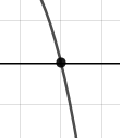
\includegraphics[width = 0.3\textwidth]{../Figures/polyZeroBehaviorAC.png}\item 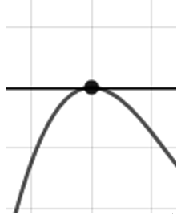
\includegraphics[width = 0.3\textwidth]{../Figures/polyZeroBehaviorBC.png}\item 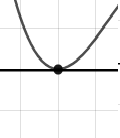
\includegraphics[width = 0.3\textwidth]{../Figures/polyZeroBehaviorCC.png}\item 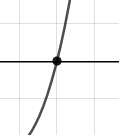
\includegraphics[width = 0.3\textwidth]{../Figures/polyZeroBehaviorDC.png}\end{multicols}\item None of the above.
\end{enumerate} }
\litem{
Describe the end behavior of the polynomial below.\[ f(x) = -3(x - 5)^{2}(x + 5)^{3}(x - 8)^{5}(x + 8)^{6} \]\begin{enumerate}[label=\Alph*.]
\begin{multicols}{2}\item 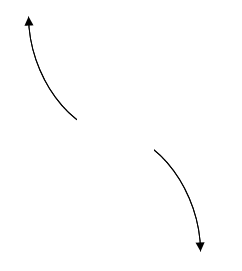
\includegraphics[width = 0.3\textwidth]{../Figures/polyEndBehaviorAC.png}\item 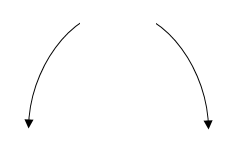
\includegraphics[width = 0.3\textwidth]{../Figures/polyEndBehaviorBC.png}\item 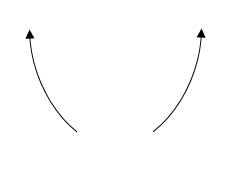
\includegraphics[width = 0.3\textwidth]{../Figures/polyEndBehaviorCC.png}\item 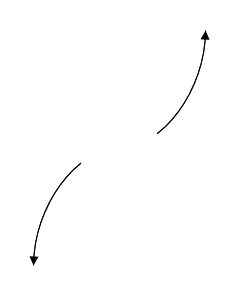
\includegraphics[width = 0.3\textwidth]{../Figures/polyEndBehaviorDC.png}\end{multicols}\item None of the above.
\end{enumerate} }
\litem{
Describe the zero behavior of the zero $x = 5$ of the polynomial below.\[ f(x) = 3(x - 4)^{8}(x + 4)^{7}(x - 5)^{14}(x + 5)^{9} \]\begin{enumerate}[label=\Alph*.]
\begin{multicols}{2}\item 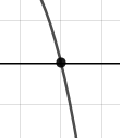
\includegraphics[width = 0.3\textwidth]{../Figures/polyZeroBehaviorCopyAC.png}\item 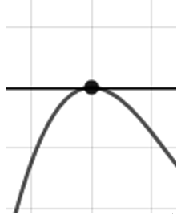
\includegraphics[width = 0.3\textwidth]{../Figures/polyZeroBehaviorCopyBC.png}\item 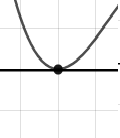
\includegraphics[width = 0.3\textwidth]{../Figures/polyZeroBehaviorCopyCC.png}\item 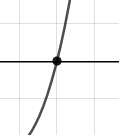
\includegraphics[width = 0.3\textwidth]{../Figures/polyZeroBehaviorCopyDC.png}\end{multicols}\item None of the above.
\end{enumerate} }
\litem{
Describe the end behavior of the polynomial below.\[ f(x) = 4(x + 7)^{2}(x - 7)^{5}(x - 6)^{2}(x + 6)^{4} \]\begin{enumerate}[label=\Alph*.]
\begin{multicols}{2}\item 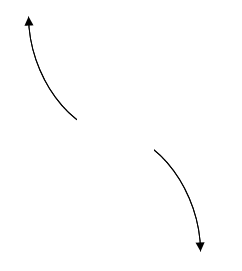
\includegraphics[width = 0.3\textwidth]{../Figures/polyEndBehaviorCopyAC.png}\item 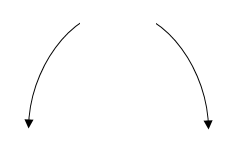
\includegraphics[width = 0.3\textwidth]{../Figures/polyEndBehaviorCopyBC.png}\item 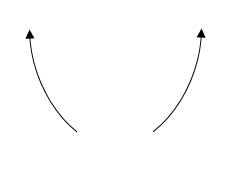
\includegraphics[width = 0.3\textwidth]{../Figures/polyEndBehaviorCopyCC.png}\item 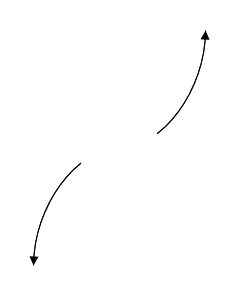
\includegraphics[width = 0.3\textwidth]{../Figures/polyEndBehaviorCopyDC.png}\end{multicols}\item None of the above.
\end{enumerate} }
\litem{
Construct the lowest-degree polynomial given the zeros below. Then, choose the intervals that contain the coefficients of the polynomial in the form $x^3+bx^2+cx+d$.\[ -4 + 4 i \text{ and } -3 \]\begin{enumerate}[label=\Alph*.]
\item \( b \in [1, 4], c \in [0, 11], \text{ and } d \in [12, 13] \)
\item \( b \in [1, 4], c \in [-4, 2], \text{ and } d \in [-16, -4] \)
\item \( b \in [6, 13], c \in [54, 60], \text{ and } d \in [89, 97] \)
\item \( b \in [-13, -8], c \in [54, 60], \text{ and } d \in [-97, -90] \)
\item \( \text{None of the above.} \)

\end{enumerate} }
\litem{
Construct the lowest-degree polynomial given the zeros below. Then, choose the intervals that contain the coefficients of the polynomial in the form $x^3+bx^2+cx+d$.\[ 4 + 2 i \text{ and } -4 \]\begin{enumerate}[label=\Alph*.]
\item \( b \in [0.3, 1.4], c \in [1.4, 6.2], \text{ and } d \in [-12, -6] \)
\item \( b \in [-7.4, -2], c \in [-12.6, -9.7], \text{ and } d \in [79, 85] \)
\item \( b \in [3.9, 6.7], c \in [-12.6, -9.7], \text{ and } d \in [-83, -73] \)
\item \( b \in [0.3, 1.4], c \in [-0.1, 0.9], \text{ and } d \in [-23, -9] \)
\item \( \text{None of the above.} \)

\end{enumerate} }
\litem{
Which of the following equations \textit{could} be of the graph presented below?
\begin{center}
    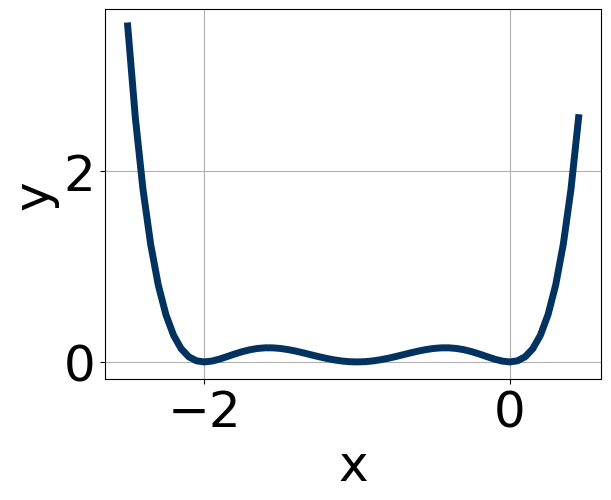
\includegraphics[width=0.5\textwidth]{../Figures/polyGraphToFunctionCopyC.png}
\end{center}
\begin{enumerate}[label=\Alph*.]
\item \( 15(x - 2)^{7} (x + 1)^{6} (x + 2)^{9} \)
\item \( -15(x - 2)^{6} (x + 1)^{5} (x + 2)^{11} \)
\item \( 11(x - 2)^{4} (x + 1)^{8} (x + 2)^{11} \)
\item \( -18(x - 2)^{4} (x + 1)^{11} (x + 2)^{10} \)
\item \( 6(x - 2)^{4} (x + 1)^{11} (x + 2)^{7} \)

\end{enumerate} }
\litem{
Construct the lowest-degree polynomial given the zeros below. Then, choose the intervals that contain the coefficients of the polynomial in the form $ax^3+bx^2+cx+d$.\[ \frac{4}{3}, -3, \text{ and } \frac{4}{5} \]\begin{enumerate}[label=\Alph*.]
\item \( a \in [15, 17], b \in [-14, -5], c \in [-84, -73], \text{ and } d \in [-50, -47] \)
\item \( a \in [15, 17], b \in [6, 16], c \in [-84, -73], \text{ and } d \in [-50, -47] \)
\item \( a \in [15, 17], b \in [52, 62], c \in [5, 13], \text{ and } d \in [-50, -47] \)
\item \( a \in [15, 17], b \in [-41, -33], c \in [-42, -35], \text{ and } d \in [43, 55] \)
\item \( a \in [15, 17], b \in [6, 16], c \in [-84, -73], \text{ and } d \in [43, 55] \)

\end{enumerate} }
\litem{
Which of the following equations \textit{could} be of the graph presented below?
\begin{center}
    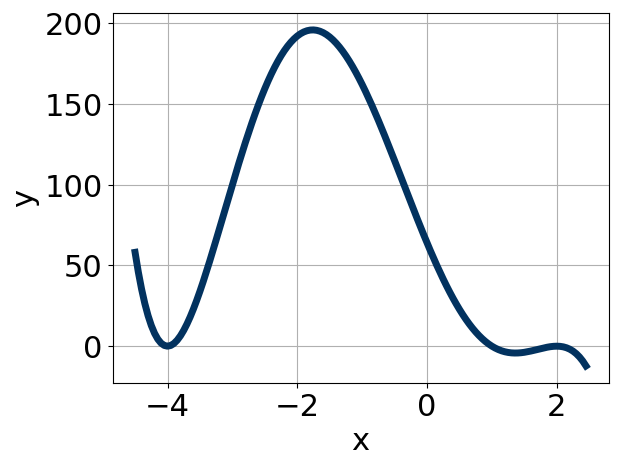
\includegraphics[width=0.5\textwidth]{../Figures/polyGraphToFunctionC.png}
\end{center}
\begin{enumerate}[label=\Alph*.]
\item \( 7x^{9} (x + 4)^{11} (x + 3)^{11} \)
\item \( 11x^{9} (x + 4)^{6} (x + 3)^{7} \)
\item \( -17x^{11} (x + 4)^{8} (x + 3)^{11} \)
\item \( -15x^{5} (x + 4)^{9} (x + 3)^{5} \)
\item \( 14x^{11} (x + 4)^{4} (x + 3)^{4} \)

\end{enumerate} }
\end{enumerate}

\end{document}